\section{Background}
%Optimization
Nowadays, 
it has become easy to obtain  enormous computational resources, and
one kind of the most interesting challenges is
to apply computational techniques towards complex problems.
The computational optimization is  
an effective and essential technique for dealing with complex problems.
There are many optimization methods such as
branch and bound methods, gradient methods, Newton methods, simulated
annealing methods, and mean field annealing methods.

 
%Evolution
Evolutionary algorithms (EAs) such as genetic algorithms (GAs) 
\cite{goldberg:ga,weise:go}
are comparatively new optimization techniques.
Since they have a relatively short history,
EAs have not been widely employed and 
the fundamental principle have not been established yet.
However, substantial studies on EAs have been carried out energetically
and they have steadily contributed to reveal
the essential mechanism of EAs.
Consequently, we have one promising approach in sight now.


%EAPM
Actually, this approach have not possessed the official name and, 
in fact, the official definition have not been established yet.
At least, it has been well confirmed that 
the essential key technique is statistical estimation.
In general, estimation of the cost function is 
important task in computational optimization.
For example, the Newton method predicts
the cost function by using Taylor expansion.
On the other hand, in the focused approach,
statistical estimation predicts the structure of 
the cost function instead of Taylor expansion.
This is clearly new approach.


This approach attracted attentions for the first time
when the works of M\"{u}hlenbein
\cite{muhlenbein:umda,muhlenbein:umda_c}
appeared.
It should be noted that there were similar studies such as
\cite{baluja:pbil} before them.
Methods inspired by this approach are called
estimation of distribution algorithms (EDAs). 
Actually, 
EDAs are intended to be a mathematical model of GAs
and someone call methods based on this approach
probabilistic model-building genetic algorithms (PMBGAs)
\cite{pelikan:pmbga}.
Surprisingly, in a different field, that is, rare event simulation,
a similar approach is proposed by Rubinstein 
as one of the Monte Carlo integration techniques and
named the cross entropy method (CE) \cite{rubinstein:ce}.
Currently, 
it has become well known that
the three different names share the common and essential
concept, that is, statistical estimation of the distribution of
promising solutions, 
and the common name, evolutionary algorithms based on probability models
(EAPM), is proposed 
in the congress on evolutionary computation (CEC) in 2007.
This thesis uses this name.

%What is EAPM
One advantage of EAPM to other EAs is
the mathematical definition of the algorithms.
In EAPM, an objective is statistically estimation of
promising solutions from the past samples.
This problem setting can be defined mathematically 
and we can develop EAPM in theoretical manners.
Recent studies on EAPM \cite{larranaga:eda} mainly improve the
statistical estimation, for example,
employing complex probability models such as Bayesian networks.


\section{Objectives and Contributions}
The essential mechanism of EAPM consists of two techniques:
statistical estimation and additionally Monte Carlo integration (MCI).
Statistical estimation plays the central role in EAPM.
On the other hand, MCI has an effect on the estimation accuracy.
This thesis focuses not on the aspect of statistical estimation
but on the aspect of Monte Carlo integration,
whereas almost studies on EAPM focuses on 
statistical estimation methods.

This thesis improves the Monte Carlo integration of EAPM
in three directions.
%abst
First, this thesis proposes a novel technique,
resampling population model (RPM),
for reusing the historical samples.
The difficulty of employing the historical samples is
that
simply selecting good historical samples causes 
the bias of the statistical estimation.
RPM weights the historical samples
in terms of importance sampling 
for possibly removing the bias.

Second,
this thesis focuses on the convergence mechanism.
In general EAPM,
highly random sampling is employed in early stages,
and the randomness is gradually decreased.
Finally, the sampler distribution converges a point.
This mechanism involves the problem of local optima
because there is no opportunity to escape from local optima after convergence.
To overcome this problem,
this thesis proposes a novel method,
hierarchical importance sampling (HIS) which mixes 
samples with different randomness.
In other words, highly random sampling, slightly random sampling, and
converged sampling are carried out simultaneously.
Higher randomness contributes to escape from local optima
and, in this method, high randomness is employed at all stages.
The difficulty is to retrieve information from mixed samples.
HIS overcomes this difficulty by using 
importance sampling with a mixture distribution.
By using this technique, information can be retrieved from mixed samples
in a theoretically valid manner.
This method is also related to multi-start method.

Third,
this thesis proposes a novel convergence schedule.
In EAPM,
it is important not only to control the convergence speed
but also to determine its speed.
Actually, there is no convergence schedule with theoretical discussions.
This thesis reveals the relationship between
the randomness of the target distribution
(i.e., the ideal sampler distribution 
which guides where samples should be generated)
and the accuracy of the statistical estimation,
that is,
the entropy of the target distribution and the Fisher information.
As a result, we obtain an approximately optimal convergence schedule
, entropy reduction schedule (ERS),
where the entropy of the target distribution
is linearly reduced.
This implies that the algorithm converges in linear time for a problem
with
an exponential size of the search space.

Consequently, this thesis extends
the basic framework of EAPM in new two directions:
(1)mixing current and  historical samples,
 and (2)mixing samples with different randomness.
On the other hand, the convergence schedule is an essential element of
EAPM and the overall improvement can be expected.
The brief relationship is shown in Fig. \ref{intro-relation}.
The aim of this thesis is to confirm 
the effectiveness of each improvement through experiments
and
additionally, 
with advanced benchmark problems such as Rosenbrock and Rastrigin function,
to reveal comprehensive properties of RPM and HIS:
(1) RPM has the robustness 
against the instability of the statistical estimation and 
(2) HIS has the robustness against local optima.
\begin{figure}[tbp]
\centerline{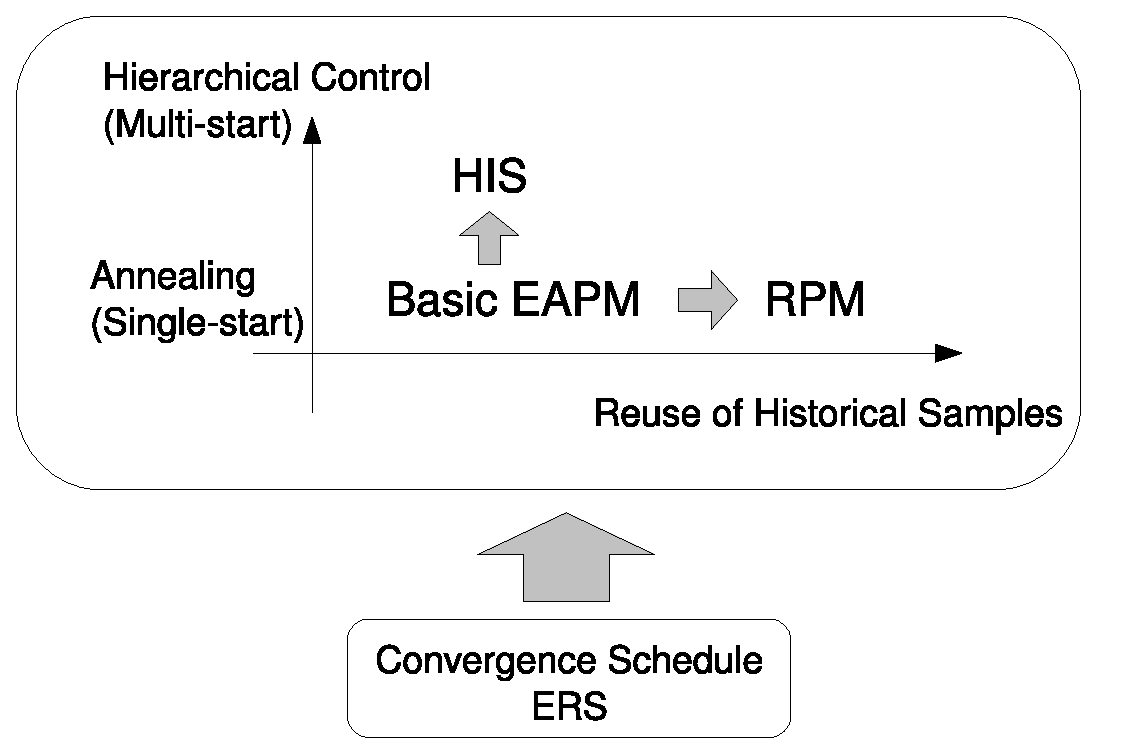
\includegraphics[width=\figlength\linewidth]{data_intro/relation.eps}}
\caption{Relationship among the proposed methods.}
\label{intro-relation}
\end{figure}

 
\section{Outline}
This thesis is organized as follows:
Chapter \ref{chapter-preliminary} introduces basic knowledge such as computational optimization,
Monte Carlo integration and statistical estimation,
and 
Chapter \ref{chapter-eapm} explains the basics of EAPM.
Chapter \ref{chapter-rpm} describes a method for using the historical samples.
Chapter \ref{chapter-his} describes a hierarchically control of the randomness of generated samples.
Chapter \ref{chapter-ers} describes a novel convergence schedule and its
theoretical aspect.
Chapter \ref{chapter-aexp} conducts advanced experiments to investigate
comprehensive properties of RPM and HIS through discrete and continuous 
problems.
Chapter \ref{chapter-conclusion} summarizes the results and concludes this thesis.
